\documentclass[12pt, twoside]{article}

\usepackage{amsfonts}
%\usepackage[T1]{fontenc}
%\usepackage[ansinew]{inputenc}
\usepackage{amssymb}
\usepackage{amsthm}
\usepackage{amsmath}
\usepackage{dsfont}
\usepackage{natbib}
\setlength{\bibsep}{0pt plus 100ex}
\usepackage{url}
\usepackage{pdflscape}
\usepackage{pdfpages}
\usepackage{svg}
\usepackage[utf8]{inputenc}
\usepackage{graphicx}


\usepackage{enumitem}
%\usepackage[german,  onelanguage, linesnumbered]{algorithm2e}
\usepackage{placeins}
\usepackage{a4}
\usepackage[a4paper, ]{geometry}
\geometry{
 a4paper,
 right=30mm,
 left=30mm,
 top=30mm,
 }

% For tables
\usepackage{tabularx}
\usepackage{multirow}
\usepackage{pbox}

% \usepackage{color}

\widowpenalty = 5000
\clubpenalty = 5000


\newcommand{\Prob}{\mathbb{P}}
\newcommand{\V}{\mathbb{V}}
\newcommand{\Cov}{\text{Cov}}
\newcommand{\E}{\mathbb{E}}
\newcommand{\R}{\mathbb{R}}
\newcommand{\1}{\mathbb{1}}
\newcommand{\LL}{\mathcal{L}}
\newcommand{\F}{\mathcal{F}}
\newcommand{\iid}{\overset{\text{iid}}{\sim}}
\newcommand{\SUM}{\sum_{i=1}^n}
\newcommand{\PROD}{\prod_{i=1}^n}



\begin{document}

\begin{titlepage}

    \newcommand{\HRule}{\rule{\linewidth}{0.5mm}} % Defines a new command for the horizontal lines, change thickness here

    \center % Center everything on the page
 
    %----------------------------------------------------------------------------------------
    %	HEADING SECTIONS
    %----------------------------------------------------------------------------------------
    
\includegraphics[scale = 0.22]{campus-seal.jpg}\\[0.5cm]
    
     \textsc{\large University of California, los Angeles}\\[0.2cm] % Minor heading such as course title
     \textsc{\large Department of Statistics}\\[0.5cm]
    %----------------------------------------------------------------------------------------
    %	TITLE SECTION
    %----------------------------------------------------------------------------------------

    \HRule \\[0.4cm]
    { \huge \bfseries Principal-Component-Wise Bootstrap}\\[0.2cm] % Title of your document
    \HRule \\[0.4cm]
    \textsc{\large An Orthogonal Spin on the Classic}\\[2.0 cm]
 
    %----------------------------------------------------------------------------------------
    %	AUTHOR SECTION
    %----------------------------------------------------------------------------------------
    
    	\hspace{1cm}
    \begin{minipage}{0.4\textwidth}
    \begin{flushleft} \large
    \emph{Authors:}\\
        Harrison \textsc{Katz} \\
        Thomas \textsc{Maierhofer} % Your name
    \end{flushleft}
    \end{minipage}
    ~
    \begin{minipage}{0.4\textwidth}
    \begin{flushright} \large
    \emph{Stats 201B:} \\
    Winter Quarter 2019,
    Prof. Chad Hazlett % Supervisor's Name
    \end{flushright}
    \end{minipage}\\[2cm]
    
    \large{
    Final Project Report
    } \\[2cm]
    
    {\large March 22, 2019}\\[2cm] % Date, change the \today to a set date if you want to be precise

    %----------------------------------------------------------------------------------------

    \vfill % Fill the rest of the page with whitespace

\end{titlepage}

%\newpage
%\hspace{5cm}
%\newpage

\pagenumbering{roman}
\tableofcontents 
\clearpage

\begin{abstract}
TODO
\end{abstract}
\clearpage
\pagenumbering{arabic}

\section{Background}
\subsection{$p$ Norms for Vectors}
This section formally introduces $p$ norms with a focus on the special cases $ p = 0, 1, 2, \infty$.
The $p$ norm of a vector $x \in \R^d$ is denoted as $||x||_p$ and defined as
$$||x||_p = \left(\sum_{i = 1}^d |x_i|^p \right)^{1/p},$$
where $|x_i| = \text{sign}(x_i)x_i$ denotes the absolute value. In literature $p$ norms are often denoted as $l_p$ norms.

The most important special cases is the $2$ norm, a.k.a.\ Euclidean norm. It is defined as
$$||x||_2 = \sqrt{\sum_{i = 1}^d x_i^2}.$$
Other important cases include the $0$ norm,
$$||x||_0 = \sum_{i = 1}^d \1\{x_i \neq 0\},$$
the $1$ norm, a.k.a.\ Manhattan norm,
$$||x||_1 = \sum_{i = 1}^d |x_i|,$$
and the $\infty$ norm, a.k.a. maximum norm,
$$||x||_\infty = \max_{i = 1, \ldots, d} |x_i|.$$

A unit ball for a norm $||\cdot||$ contains all points with distance $1$ around the origin, i.e. all points $\{x: ||x|| = 0\}$. The unit balls for the $1, 2,$ and $\infty$ norm in $\R^2$ are depicted in Figure~\ref{fig:input}.
\begin{figure}[ht]
    \centering
    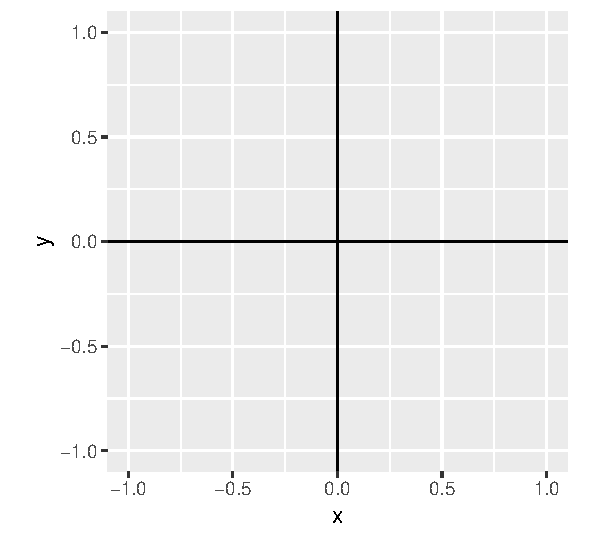
\includegraphics[width=0.49\textwidth]{plots/unit_circle_0.pdf}
    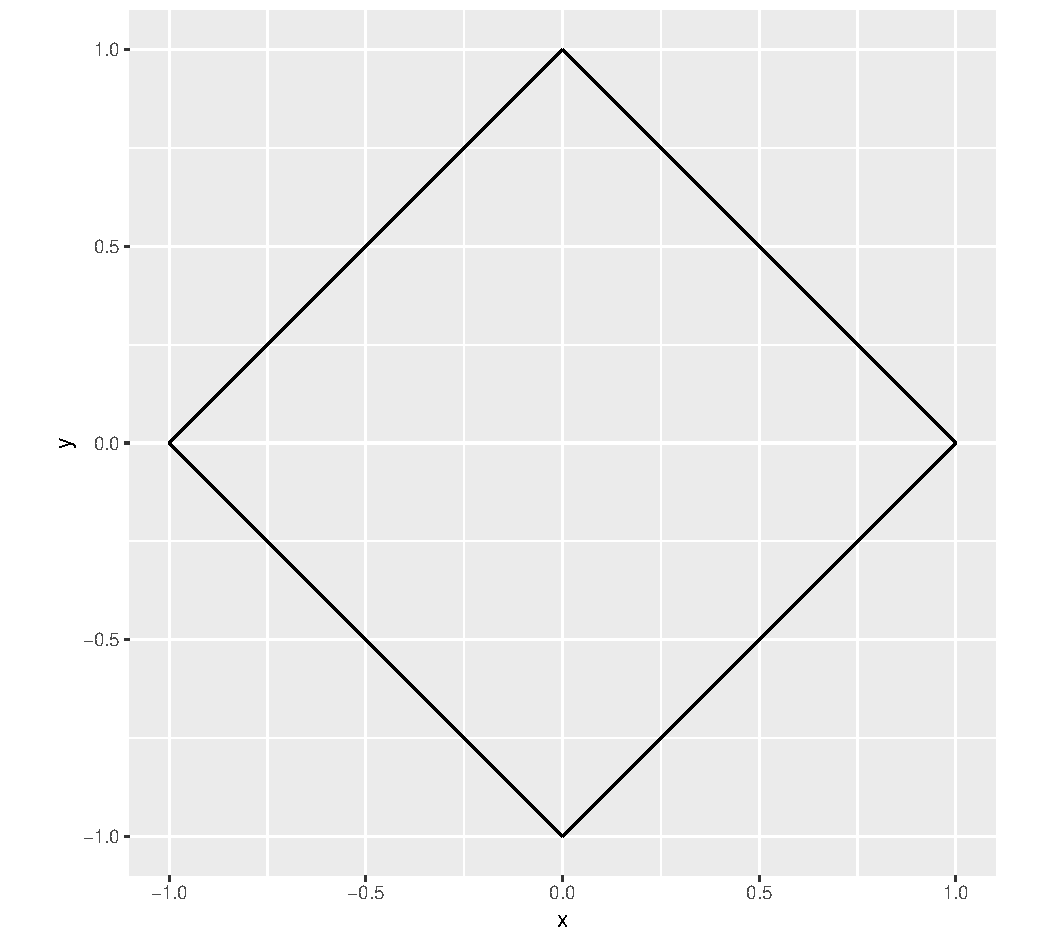
\includegraphics[width=0.49\textwidth]{plots/unit_circle_1.pdf}
    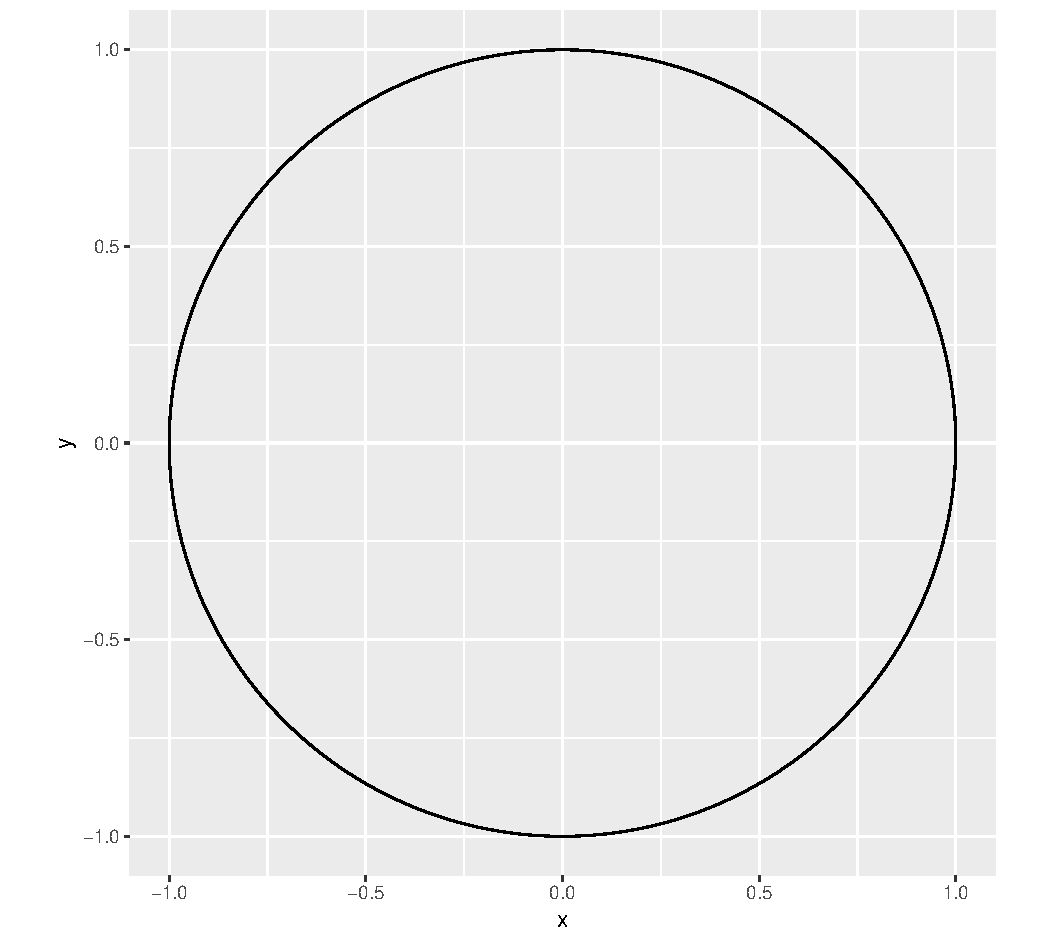
\includegraphics[width=0.49\textwidth]{plots/unit_circle_2.pdf}
    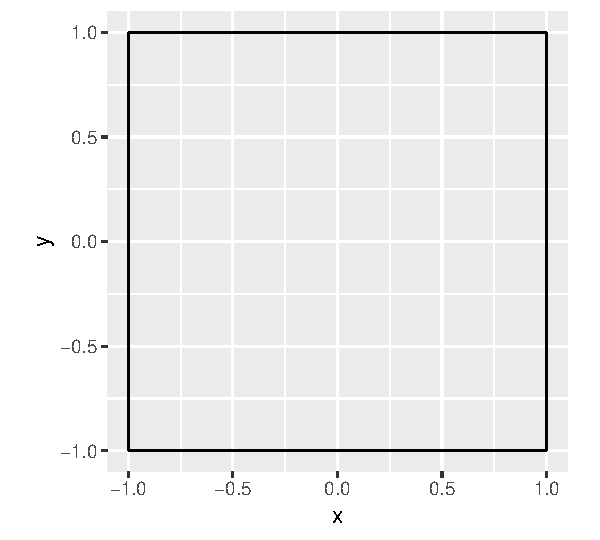
\includegraphics[width=0.49\textwidth]{plots/unit_circle_inf.pdf}
    \caption{Unit balls in $\R^2$ of the $l_0$ (topleft), $l_1$ (topright), $l_2$ (bottom left), an $l_\infty$ norm (bottom right).}
    \label{fig:input}
\end{figure}


%%%%%%%%%%%%%%%%%%%%%%%%%%%%%%%%%%%%%%%%%%%%%%%%%%%%%%%%%%%%%%%%%%%%%
\clearpage
\bibliographystyle{dcu} 
{\bibliography{bibliography.bib}}
\nocite{maierhoferCoFD}

%%%%%%%%%%%%%%%%%%%%%%%%%%%%%%%%%%%%%%%%%%%%%%%%%%%%%%%%%%%%%%%%%%%%%
% appendix

\end{document}